\chapter{Backgrounds}
\label{sec:Backgrounds}

The big disadvantage of semileptonic decays is that the neutrino can't be reconstructed.
At hadron colliders like the \lhc is it impossible to know the initial state, so one doesn't have enough constraints to reconstruct the full kinematic information about the decaying particle.
Being aware of these problems due to experimental setup it is clear that one can't use a well reconstructed \Lb mass peak to separate signal from background.
A main source of background is expected to be the decay \decay{\Bd/\Bp}{\Dz\mun\neumb X} where one randomly combines a proton to this decay.
Ths background is handled by the fit of the \logIP distribution.
Other sources of backgrounds and their possible impact on the obtained signal yield \NDp are discussed in the following.
For the \LbToLcmunu channel it is assumed, that all non-negligible backgrounds are accounted for due to the sidebandsubtraction and including wrong sign events as well as resonant modes components in the fit.
The discussion in this chapter thus refers completely to the \LbToDpmunuX channel.

% ====================================
% section: proton misidentification
% ====================================
\section{Proton misidentification}
A possible source of backgrounds is that one misinterprets a decay as \LbToDpmunuX since one misidentifies a final state particle.
In this analysis it is most likely that the proton is misidentified since the final state pion and kaon are reconstructed to a \Dz yielding in a nice peak and the muon leaves a clear signature in the detector due to its relatively long lifetime and low interaction with matter.
Examples for these kind of backgrounds are the decays \decay{\Bs}{\Dz\Kp\mun\neumb X} and \decay{\Bd/\Bp}{\Dz\pip\mun\neumb X}, where either the \Kp or \pip is misidentified as proton.
Though there are tight requirements on the proton identification at selection stage, the data will still be polluted by misidentified particles.
To identify the amount of misidentified protons, a slightly different data sample than the nominal one is used. 
In this sample no requirements on the proton idenfication are applied.
Except for those all other requirements are the same as described in section \ref{sec:Selection}.
However the removal of the particle identification requirements lets the data size of the sample rapidly increase.
To keep the data size acceptable a so called 5\% prescaling has been applied, i.e. only 5\% of all events are actually stored.
The decision if a particle is stored or not is made by random.
The study on misidentified backgrounds is done in three steps.

\subsection{Definition of PID particle regions - Number of particle candidates}
As a first step we define PID regions for protons, pions and kaons in the PIDK vs. PIDp plane. 
The proton region is motivated by the cuts applied in the analysis. In detail these are:
\begin{itemize}
\item proton: $\text{PIDp} - \text{PIDK} > 10.0 \text{ and } \text{PIDp} > 10.0$
\item pion: $\text{PIDp} < 10.0 \text{ and } \text{PIDK} < 0.0$
\item kaon: $\text{PIDp} - \text{PIDK} < 10.0 \text{ and } \text{PIDK} > 0.0$
\end{itemize}

Furthermore these regions and their population are visualised in figure \ref{fig:PIDregions}. From this we get the number of candidates for each particle species, in the following denoted as \Ncand{i}, with $i \in \left[\pi, \kaon, \proton\right]$. The number of candidates are
\begin{align}
    \Ncand{\pi} = \PIDNcandpionval \pm \PIDNcandpionerr, \\ 
    \Ncand{\kaon} = \PIDNcandkaonval \pm \PIDNcandkaonerr, \\ 
    \Ncand{\proton} = \PIDNcandprotonval \pm \PIDNcandprotonerr 
\end{align}

\begin{figure}[hptb]
	\centering
	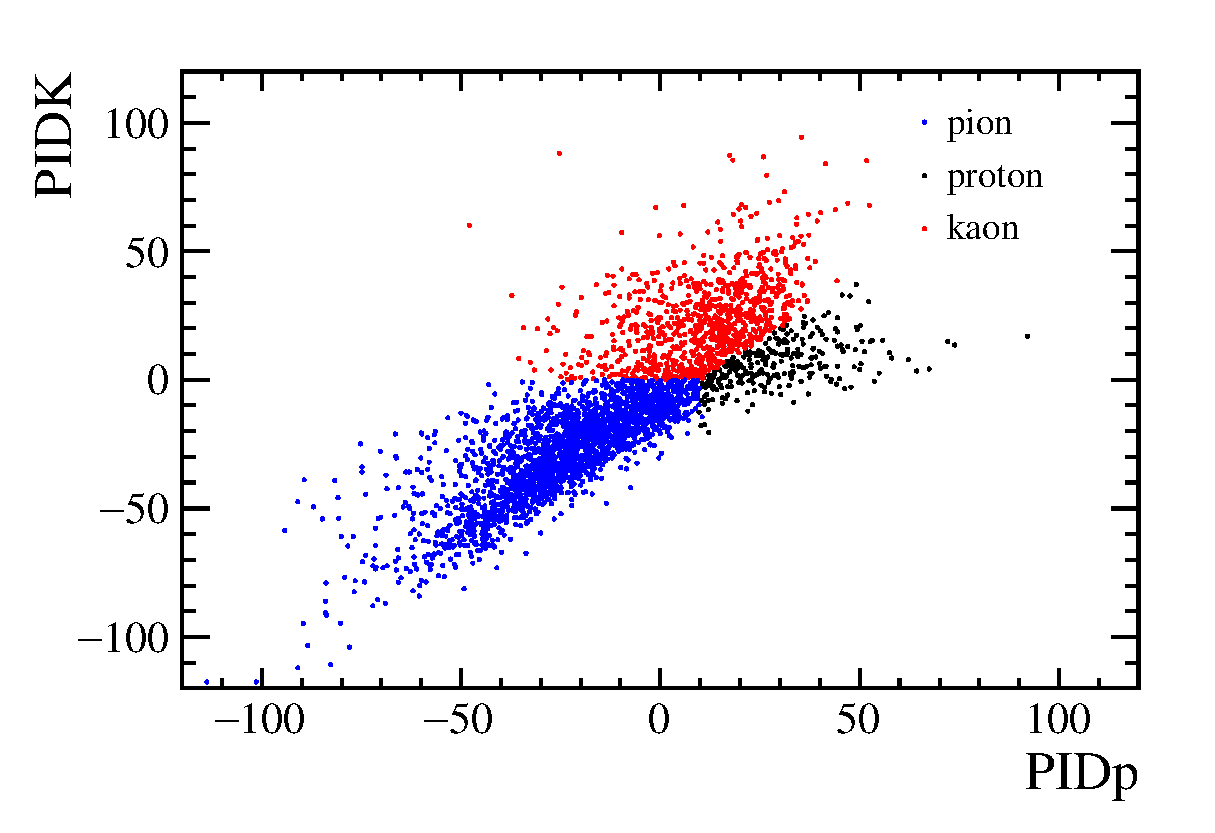
\includegraphics[width=0.49\textwidth]{LbToD0p/PID/PIDK_vs_PIDp}
	\caption{Regions for the number of particle candidates.}
	\label{fig:PIDregions}
\end{figure}


\subsubsection{Determination of ``true" candidates with PID efficiencies}
The \lhcb PIDcalib tool is used to determine the PID efficiencies, that a real proton (or kaon / pion) is identified as what we call a proton, pion or kaon according to our defined PID regions.
The PID efficiency for each of the 9 combinated is determined binwise depending on the particle momentum. The results can be seen in figure \ref{fig:PIDefficiencies}.

\begin{figure}[hptb]
	\centering
	\includegraphics[width=0.32\textwidth]{LbToD0p/PID/PID_proton}
	\includegraphics[width=0.32\textwidth]{LbToD0p/PID/PID_kaon}
	\includegraphics[width=0.32\textwidth]{LbToD0p/PID/PID_pion}
	\caption{Efficiencies determined with PIDcalib.}
	\label{fig:PIDefficiencies}
\end{figure}

To determine a final value for each efficiency, the histograms are weighted w.r.t. the kinematic distribution of our data sample. The result is:
\begin{align*}        
\begin{pmatrix}
    \effPID{\pip}{\pip}    & \effPID{\Km}{\pip}    & \effPID{\proton}{\pip} \\
    \effPID{\pip}{\Km}     & \effPID{\Km}{\Km}     & \effPID{\proton}{\Km} \\
    \effPID{\pip}{\proton} & \effPID{\Km}{\proton} & \effPID{\proton}{\proton} 
\end{pmatrix}
=
\begin{pmatrix}
0.9409 & 0.0241 & 0.1309 \\
 0.0474 & 0.9681 & 0.3798 \\
 0.0117 & 0.0077 & 0.4893
\end{pmatrix}
\end{align*}


Here, \effPID{i}{j} denotes the efficiency, that a real particle $i$ is identified as what we call $j$. 
For the following analysis, PID efficiency errors are assumed to be negligible compared to the corresponding uncertainties of the particle candidates \Ncand{i}.
With the PID efficiencies \effPID{i}{j} and the number of particle candidates \Ncand{k}, the number of ``true" particles is determined by solving the matrix equation

\begin{align*}
    \begin{pmatrix} 
        \Ncand{\pi} \\ \Ncand{\kaon} \\ \Ncand{\proton}
    \end{pmatrix}
    =
    \begin{pmatrix}
       \effPID{\pi}{\pi}     & \effPID{\kaon}{\pi}     & \effPID{\proton}{\pi} \\
       \effPID{\pi}{\kaon}   & \effPID{\kaon}{\kaon}   & \effPID{\proton}{\kaon} \\
       \effPID{\pi}{\proton} & \effPID{\kaon}{\proton} & \effPID{\proton}{\proton} 
    \end{pmatrix}
    \begin{pmatrix} 
        \Ntrue{\pi} \\ \Ntrue{\kaon} \\ \Ntrue{\proton }
    \end{pmatrix},
\end{align*}

which delivers
\begin{align}
    \Ntrue{\pi}     = \PIDNtruepionval \pm \PIDNtruepionerr, \\ 
    \Ntrue{\kaon}   = \PIDNtruekaonval \pm \PIDNtruekaonerr, \\ 
    \Ntrue{\proton} = \PIDNtrueprotonval \pm \PIDNtrueprotonerr 
\end{align}


\subsubsection{Estimate of misidentified protons}
Using the results of the previous subsections it is possible to estimate the number of misidentified protons (``true" kaons or pions identified as a proton) by multiplying the number of ``true" particles \Ntrue{i} with the PID efficiency \effPID{i}{\proton} to be identified as proton. 
\begin{align}
    N^{\pi} = \effPID{\pi}{\proton} \Ntrue{\pi}             = \PIDNtruePregionpionval \pm \PIDNtruePregionpionerr, \\  
    N^{\kaon} = \effPID{\kaon}{\proton} \Ntrue{\kaon}       = \PIDNtruePregionkaonval \pm \PIDNtruePregionkaonerr, \\ 
    N^{\proton} = \effPID{\proton}{\proton} \Ntrue{\proton} = \PIDNtruePregionprotonval \pm \PIDNtruePregionprotonerr 
\end{align}
Thus, the amount of misidentified protons is at a single-digit percent level, namely $(\misIDratioval \pm \misIDratioerr)\%$. 
Note that the absolute values can't be compared to the signal yields for both channels since this background study was done with a prescaled sample and without PID cuts.



\begin{table}
\caption{\label{tab:Backgrounds}Estimate of the residual peaking backgrounds.}
\resizebox{\textwidth}{!}{\begin{tabular}{|c|c|c|c|c|}
\hline
Mode & Estated $B/S$ & Branching fraction & Production factor & Comment \\
\hline
Signal ($\Lambda_b \rightarrow D^0 p \mu^-\nu$) & 1 & $\approx 1.5\times 10^{-3}$ & 1 & --\\
\hline
Total peaking background & 5\% & -- & -- & --\\
\hline
$\Lambda_b \rightarrow D^0 p \pi^-$ & Zero & $(5.9^{+4.0}_{-3.2})\times 10^{-4}$ & 1 & Mass veto\\
$\Lambda_b \rightarrow D^0 p \pi(\pi\pi,\pi^0)$ & 5\% & $\approx 10^{-3}$ & 1 & $\pi\rightarrow\mu$ mis-ID\\
Prompt $D^0$ & $< 10^-3$ & N/A & N/A & $\log(\mathrm{IP},D^0)$ \\ 
             &           &     &     & \& $\Lambda_b$ combination cuts\\
$B_s \rightarrow D^0 K \mu\nu X$ & $p$-misid & $\approx 6\times 10^{-3}$  & 0.5 & $p$-mis-ID\\
                                 &          & (resonant part)             &        \\
\hline
\end{tabular}}
\end{table}


The following backgrounds to the the $\Lambda_b^0 \rightarrow D^0 p \mu \nu X$ sample are considered:


\begin{itemize}
\item {\bf Prompt $D^{0}$}\\
The prompt $D^0$ cross section exceeds that of $\Lambda_b^0$ production by a factor of twenty or so.
The background from prompt charm production is typically measured to be {\bf a few percent} in studies of semileptonic $b$ decays.
Suggest to plot the distribution of the $\log(\mathrm{IP})$ of the $D^0$, which should reveal the prompt component.
This should be clearer in candidates with a wrong sign muon, or wrong sign proton, or both.
By requring a large $\log(\mathrm{IP})$ of the $D^0$, we should be able to eliminate this background althogether.
\item {\bf $B_s^{0} \rightarrow D^0 K \mu \nu X$}\\
Where the kaon is mis-identified as a proton. The mis-id rate should be a few percent, given
our tight proton PID requirements. And $f_{\Lambda_b}/f_s \sim 2$.
We should be able to estimate this contribution quite precisely just from the numbers in an early LHCb
study with 2010 data~\cite{Aaij:2011ju}.
\item {\bf $B^{0,+} \rightarrow D^0 \pi^+ \mu \nu X$}\\
Where the pion is mis-identified as a proton. The mis-id rate should be very small,
and these decays are quite well understood.
\item {\bf $B^{0,+} \rightarrow D^0 \mu \nu X$ plus a proton from the PV or other $b$}\\
This component is subtracted in our fit to the $\log(\mathrm{IP})$ of the proton w.r.t. the $D^0\mu$ vertex.
\item {\bf $\Lambda_b^0 \rightarrow D^0 p \pi X$}\\
      Where the pion is mis-identified as a muon. 
      The branching fraction of this decay has been measured to be less than $10^{-3}$. It sits in a very narrow region of $\Dz\proton\mun$ invariant mass peaking at the \Lb mass. 
      This background is eliminated by a cut on the \Dz\proton\mun mass as can be seen in figure \ref{fig:plot_D0pmuMass}.
\item {\bf \decay{\Lb}{\Dz\proton 3\pi}} \\
      The branching fraction should be similar to \decay{\Lb}{\Dz\proton\pi X}, i.e. of order $10^{-4}$. 
      The amount should decrease with increasing muon identification. 
      Figure \ref{fig:plot_D0pmuMass_vs_muPIDmu} shows a 2D plot of the \Dz\proton\muon mass versus the particle identification variable PIDmu of the muon. 
      Backgrounds coming from a \Lb decay into 3 pions should cluster at low PIDmu, where it is rather probable that a muon is misidentified than in the high PIDmu region.
\item {\bf $\Lambda_b^0 \rightarrow D \Lambda_c$}\\
      This decay hasn't been measured but it should have a branching ratio of around $10^{-2}$, similar to $B \rightarrow D D_s$.
      If the $\Lambda_c$ decays to $pK\pi$, then we get another $4 \times 10^{-2}$ and we need to get the muon from somewhere else, 
      or it has to be from $K \rightarrow \mu$ mis-id. 
      The vertex quality will be somewhat spoilt by the $\Lambda_c$ flight.
      So this should be a sub-percent-level background.
      One could also get $\Lambda_c N^* \mu \nu$, where we get the muon and proton without any mis-id?
\item {\bf $\Lambda_b^0 \rightarrow D^0 D^- p$}\\
This decay hasn't been measured but it should be similar to $B \rightarrow DDK$ at a few times $10^{-3}$.
The inclusive $D^- \rightarrow \mu^-X$ branching fraction is about $10^{-2}$.
This should still be a percent level background.
\item {\bf prompt \LcResI or \LcResII decay with an \mun from somewhere else} \\
This background should be reduced by requiring the \LcResI resp. \LcResII vertex to be well separated from the PV.
\item \textbf{ \decay{\SigmabRes}{\Lb \pi}}, where the pion isn't reconstructed.
\end{itemize}

\begin{figure}[hptb]
	\centering
	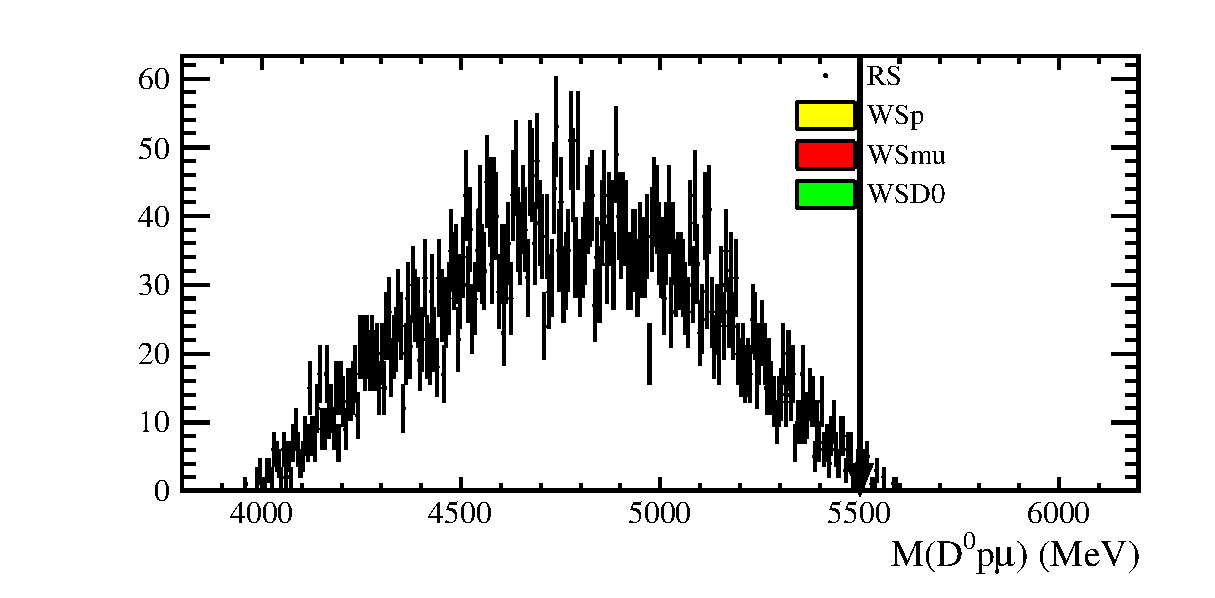
\includegraphics[width=0.49\textwidth]{LbToD0p/plots/data/Bh_M}
	\caption{Invariant \Dz\proton\mun mass. The arrow indicates the cut applied in this analysis. The peak at \Lb mass ($\approx 5620 \mev$) comes from the decay \decay{\Lb}{\Dz\proton\pi} where the pion is misidentified as muon.}
	\label{fig:plot_D0pmuMass}
\end{figure}

\begin{figure}[hptb]
	\centering
	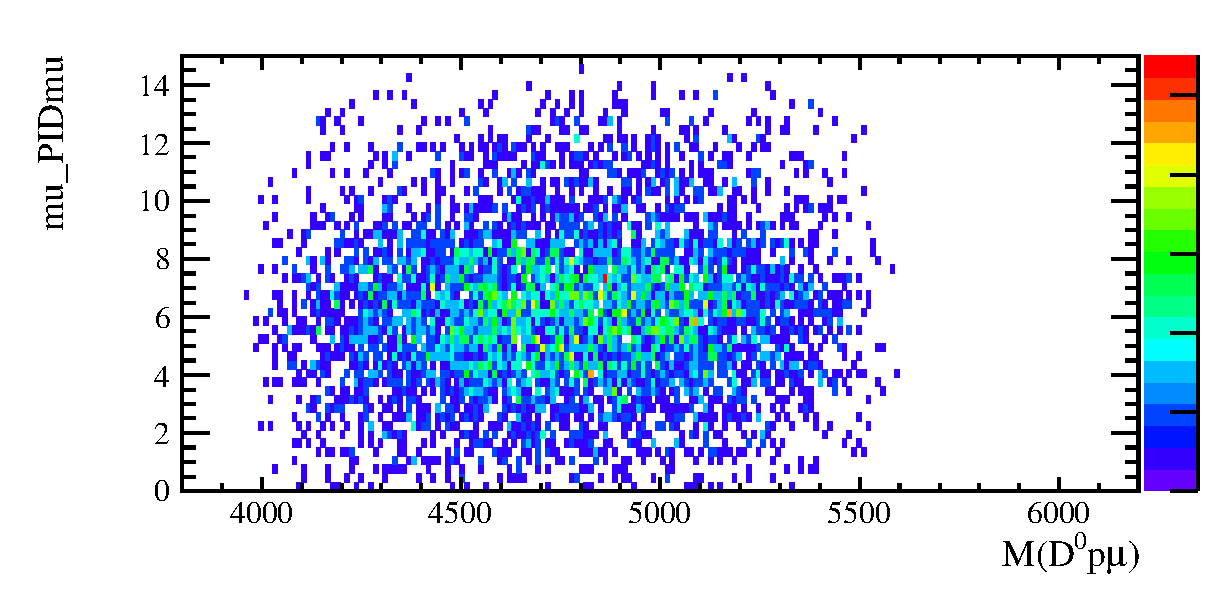
\includegraphics[width=0.49\textwidth]{LbToD0p/plots/data/Bh_M_vs_mu_PIDmu_RS}
	\caption{Invariant \Dz\proton\mun mass versus PIDmu of the muon. No structures tending to low PIDmu can be seen.}
	\label{fig:plot_D0pmuMass_vs_muPIDmu}
\end{figure}

